\documentclass[12pt]{article}
\usepackage{geometry}                % See geometry.pdf to learn the layout options. There are lots.
\geometry{letterpaper}                   % ... or a4paper or a5paper or ... 
%\geometry{landscape}                % Activate for for rotated page geometry
\usepackage[parfill]{parskip}    % Activate to begin paragraphs with an empty line rather than an indent
\usepackage{daves,fancyhdr,natbib,graphicx,dcolumn,amsmath,lastpage,url}
\usepackage{amsmath,amssymb,epstopdf,longtable}
\usepackage{paralist} 
\usepackage[final]{pdfpages}
\DeclareGraphicsRule{.tif}{png}{.png}{`convert #1 `dirname #1`/`basename #1 .tif`.png}
\pagestyle{fancy}
\lhead{CE 3372 -- Water Systems Design}
\rhead{FALL 2017}
\lfoot{ES 16}
\cfoot{}
\rfoot{Page \thepage\ of \pageref{LastPage}}
\renewcommand\headrulewidth{0pt}



\begin{document}
\begin{center}
{\textbf{{ CE 3372 -- Water Systems Design} \\ {Exercise Set 16}}}
\end{center}

\begingroup
\begin{tabular}{p{2in} p{4.5in}}
Purpose: & Apply rational method using SWMM\\
~ & ~ \\
ABET General Criteria 3: & (a) \dots apply knowledge of mathematics, science, and engineering  \\
~ & (e)  \dots solve engineering problems  \\
~ & (k) \dots an ability to use the techniques, skills, and modern engineering tools necessary for engineering practice. \\
%~ & ~ \\
%%%Grading Criteria:  & Completion; Correct Solutions; Calculation Details \\
\end{tabular}
\endgroup
\section*{\small{Exercises}}
\begin{enumerate}
%%%%%%%%%%%%%%%%%%
\item Read the attached document that explains a way to approximate the rational method in SWMM.   
\item A square shaped 50 acre, single family residential area in Harris County is graded from an elevation of 150-feet at the corner to 139-feet at the outlet as depicted on Figure \ref{fig:watershed.jpg}.

\begin{figure}[h!] %  figure placement: here, top, bottom, or page
   \centering
   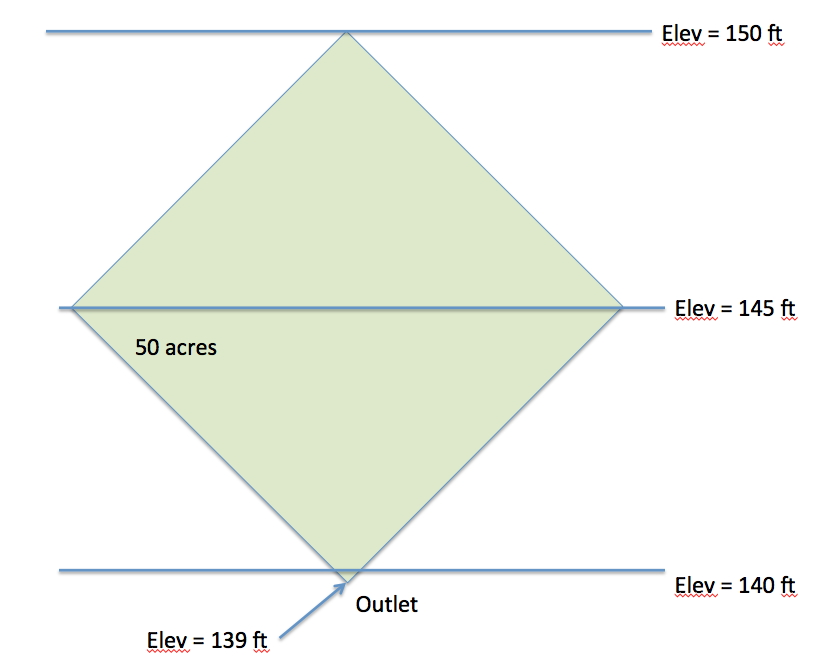
\includegraphics[width=5in]{watershed.jpg} 
   \caption{50 acre square watershed with elevation contour overlay}
   \label{fig:watershed.jpg}
\end{figure} 
\clearpage

\begin{enumerate}[a)]
\item Draw on the diagram the longest flow path from the highest elevation to the outlet.
\item Draw on the diagram the shortest flow path from the highest elevation to the outlet.
\item Determine the length, in feet, of one side (edge) of the sub-catchment.
\item Determine the length, in feet, of both flow paths.
\item Determine the average dimensionless slope along each flow path.
\item Estimate the time of concentration using NRCS upland method.
\item Using the EBDLKUP-2015 estimate the rainfall intensity for a 10-year ARI.
\item Using (and citing) a runoff coefficient table, specify the runoff coefficient for the sub-catchment.
\item Estimate the peak discharge for the sub-catchment for a 10-year ARI using the Rational Method.
\item Build a 50 acre catchment in SWMM, route runoff to an outlet node, include a raingage.
\item Build a constant-intensity storm with duration of 6 hours with the intensity equal to that you determined above.
\item Adjust the sub-catchment parameters as described in the attached document to replicate the rational method.
\item Use SWMM to simulate the runoff hydrograph from the watershed for that storm.
\item Include a screen capture of the sub-catchment dialog box where you supply sub-catchment area, and width.   
Describe how you selected your width for your model.   
\item Determine the calculated peak discharge from the SWMM model and compare its value to the value from the Rational Method.
\item Produce a memorandum that explains these steps and the resulting values.
\end{enumerate}
\end{enumerate}
\includepdf[pages={-}]{./61-HowToDoRationalInSWMM.pdf}
\end{document}  